\documentclass[../manuscript.tex]{subfiles}

\section{Обозначения, сокращения, основные определения}
\textit{В силу междисциплинарного характера данной дипломной работы, автор счел уместным определить все понятия из биологии, без которых понимание работы будет затруднено или невозможно, не вдаваясь по возможности в технические детали. Для терминов, не имеющих устоявшегося перевода на русский язык, были использованы принятые в научном сообществе транслитерации.}

\begin{definition}[\textit{Центральная догма молекулярной биологии}]$ $\\
	Наблюдаемая в природе закономерность передачи генетической информации: она распространяется от нуклеиновых кислот к белкам, вначале от ДНК к РНК в процессе \textbf{транскрипции}, а затем от РНК к белкам в процессе \textbf{трансляции}. Правило было впервые сформулировано Френсисом Криком в 1958 году. 
	\begin{figure}[H]
		\centering
		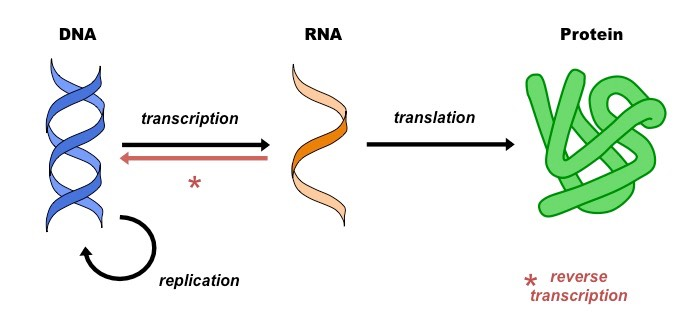
\includegraphics[keepaspectratio=true,scale=0.5]{images/central_dogma_med.jpeg}
		\caption{Центральная догма молекулярной биологии}
	\end{figure}
	В упрощённом понимании, в процессе транскрипции участок ДНК преобразуется в т.н. \textbf{пре-матричную РНК (пре-мРНК)}, которая после \textbf{сплайсинга} — вырезания \textbf{интронов}, участков, не кодирующих белковые последовательности, — превращается в \textbf{матричную РНК (мРНК)}, которая транслируется в белковую последовательность в рибосомах.
\end{definition}

\begin{definition}[\textit{Геном, экзом, транскриптом}]$  $
	\begin{enumerate}
		\item \textbf{Геном} — генетический материал клетки, нуклеотидная последовательность ДНК организма.
		\item \textbf{Экзом} — набор \textbf{экзонов} организма — участков генома, кодирующих белковые последовательности.
		\item \textbf{Транскриптом} — совокупность всех транскриптов, синтезируемых одной клеткой или группой клеток, включая мРНК и некодирующие РНК. Представляет собой ту часть экзома, которая преобразуется в белки в момент наблюдения, и зависит от типа клетки, стадии клеточного цикла, условий внешней среды и т.д.
	\end{enumerate}
\end{definition}

\begin{definition}[\textit{Референсный геном}]
	Секвенированный, собранный и проаннотированный консенсусный геном организма того же вида, к которому относится анализируемый образец.
\end{definition}

\begin{definition}[\textit{Секвенирование}]
	 Процесс определения первичной последовательности нуклеиновых кислот в клетке — ДНК или РНК. Прибор, осуществляющий секвенирование, называют \textbf{секвенатором}.
\end{definition}

\begin{definition}[\textit{Прочтение (рид)}]
	Короткий нуклеотидный фрагмент, распознанный секвенатором после ПЦР. В научном сообществе чаще используется транслитерация \textbf{\textit{рид}} от английского \textit{sequencing read}. Набор ридов, извлечённых из образца, является основным конечным продуктом секвенирования.
\end{definition}

\begin{definition}[\textit{NGS}] Next Generation Sequencing — общее название современных методов секвенирования, позволяющих, в отличие от исторических предшественников, получать полный геном, экзом или транскриптом в ходе одного эксперимента.
	\begin{figure}[H]
		\centering
		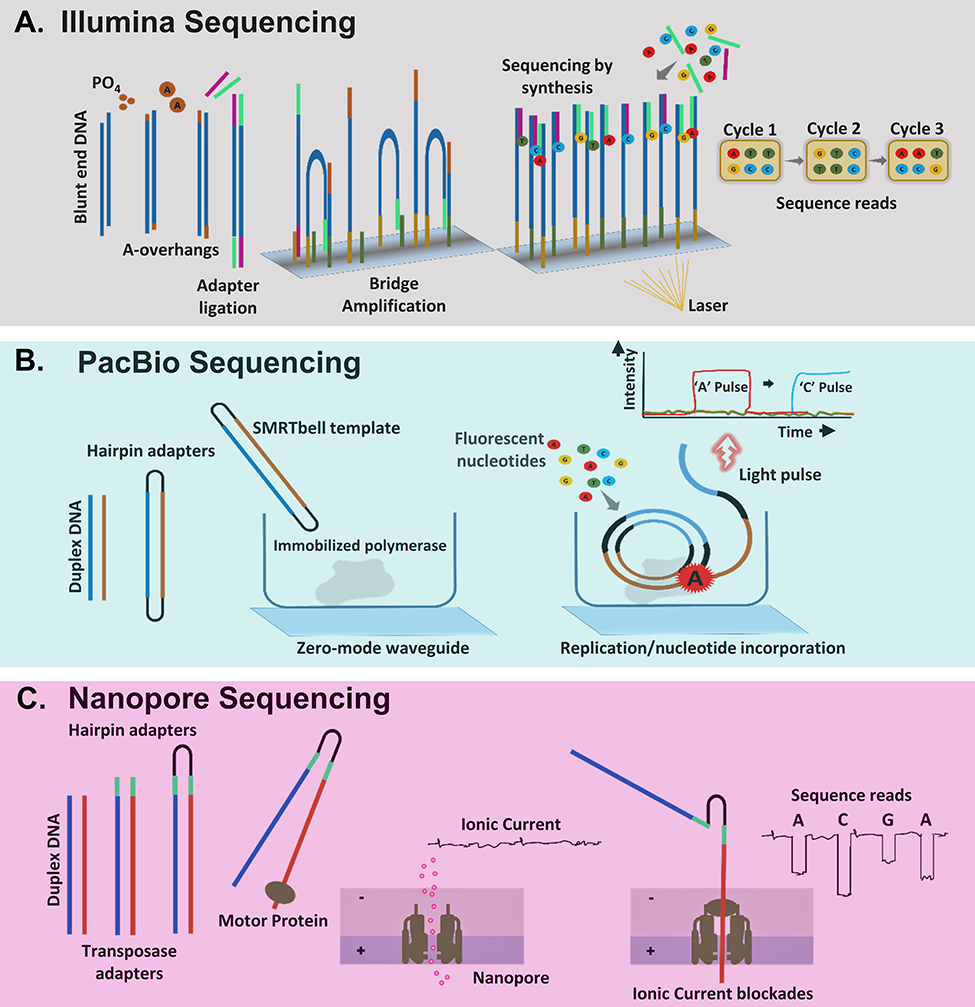
\includegraphics[keepaspectratio=true,scale=0.6]{images/ngs_types.png}
		\caption{Основные технологии высокопроизводительного секвенирования \cite{NgsReview}. В данной работе использованы данные, полученные по протоколам Illumina (1) и Oxford Nanopore (3).}
	\end{figure}
	Несмотря на то, что для обработки данных секвенирования не нужно понимать все тонкости работы секвенаторов, важно понимать, как эти технологии соотносятся. Длина ридов, полученных по технологии Oxford Nanopore, заметно больше — десятки кб против 50-300б у Illumina, — что компенсируется меньшей пропускной способностью и значительно более высокой ценой. Кроме того, нужно понимать, что при подготовке ДНК к эксперименту последняя термически или химически дробится на малые фрагменты, которые затем амплифицируются — многократно копируются при помощи специальных ферментов. То, насколько хорошо расщепляются отдельные участки ДНК, зависит от их нуклеотидного состава, и это нужно учитывать при обработке результатов.
\end{definition} 

\begin{definition}[\textit{Секвенирование одиночных клеток}]
	Совокупность новых методов секвенирования, позволяющих извлекать нуклеотидные последовательности из каждой из клеток образца в отдельности.
\end{definition}

\begin{definition}[\textit{Матрица прочтений}]
	При фиксированной сегментации генома, матрица прочтений представляет собой целочисленную матрицу, где для каждой клетки подсчитано, сколько ридов выравниваются на последовательности в пределах каждого интервала из сегментации.
\end{definition}

\begin{definition}[\textit{10X Genomics}]
	На момент написания данного текста, основной производитель технологий и программного обеспечения в нише секвенирования одиночных клеток. Представленная в работе статистическая модель проектировалась совместимой с ПО и форматом данных от 10X Genomics.
\end{definition}

\begin{definition}[\textit{ОНП (снип)}]
	Однонуклеотидный полиморфизм — позиция в геноме, на которой в статистически значимых долях популяции встречаются несколько различных вариантов нуклеотидов. Могут существенно влиять на фенотип, в том числе быть причиной патологий. В сообществе более принята траслитерация \textbf{\textit{снип}} от английского \textit{SNP — single nucleotide polymorphism}.
\end{definition}

\begin{definition}[\textit{Гетеро- и гомозиготные ОНП}]
	ОНП называется \textbf{гомозиготным}, если в родительских хромосомных наборах на соответствующей позиции находится один и тот же нуклеотид, и \textbf{гетерозиготным} в противном случае.
\end{definition}

\begin{definition}[\textit{Гаплотипирование ОНП}]
	Общее название набора методов для определения \textbf{гаплотипов} в геноме — непрерывных участков ДНК, содержащих полиморфизмы, обычно наследуемые вместе. В англоязычной литературе это называют \textit{SNP phasing}. 
\end{definition}

\begin{definition}[\textit{Ген}]
	Последовательность ДНК, составляющие сегменты которой не обязательно должны быть физически смежными. Эта последовательность ДНК содержит информацию об одном или нескольких продуктах в виде белка или РНК. Продукты гена функционируют в составе генетических регуляторных сетей, результат работы которых реализуется на уровне фенотипа.
\end{definition}

\begin{definition}[\textit{Аллель}]
	Вариант фрагмента ДНК, встречающийся в статистически значимой доле популяции. Частные случаи — ОНП, варианты генов.
\end{definition}

\begin{definition}[\textit{Аллельный дисбаланс}]
	Ситуация, когда один из аллелей доминирует над остальными — например, экспрессируется сильнее, более представлен в данных секвенирования и т.д. 
\end{definition}

\begin{definition}[\textit{CNV — структурные вариации генома}]
	\textit{CNV — copy number variation } — масштабные структурные модификации генома, такие как:
	\begin{itemize}
		\item \textbf{Loss events}:
			\subitem \textbf{Делеция} — удаление фрагмента;
		\item \textbf{Gain events}:
			\subitem \textbf{Дупликация} — удвоение фрагмента (может происходить более одного раза и порождать больше двух копий);
			\subitem \textbf{Удвоение генома} — удвоение числа хромосомных наборов;
		\item \textbf{Инверсия} — обращение непрерывного подотрезка;
	\end{itemize}
	\begin{figure}[H]
		\centering
		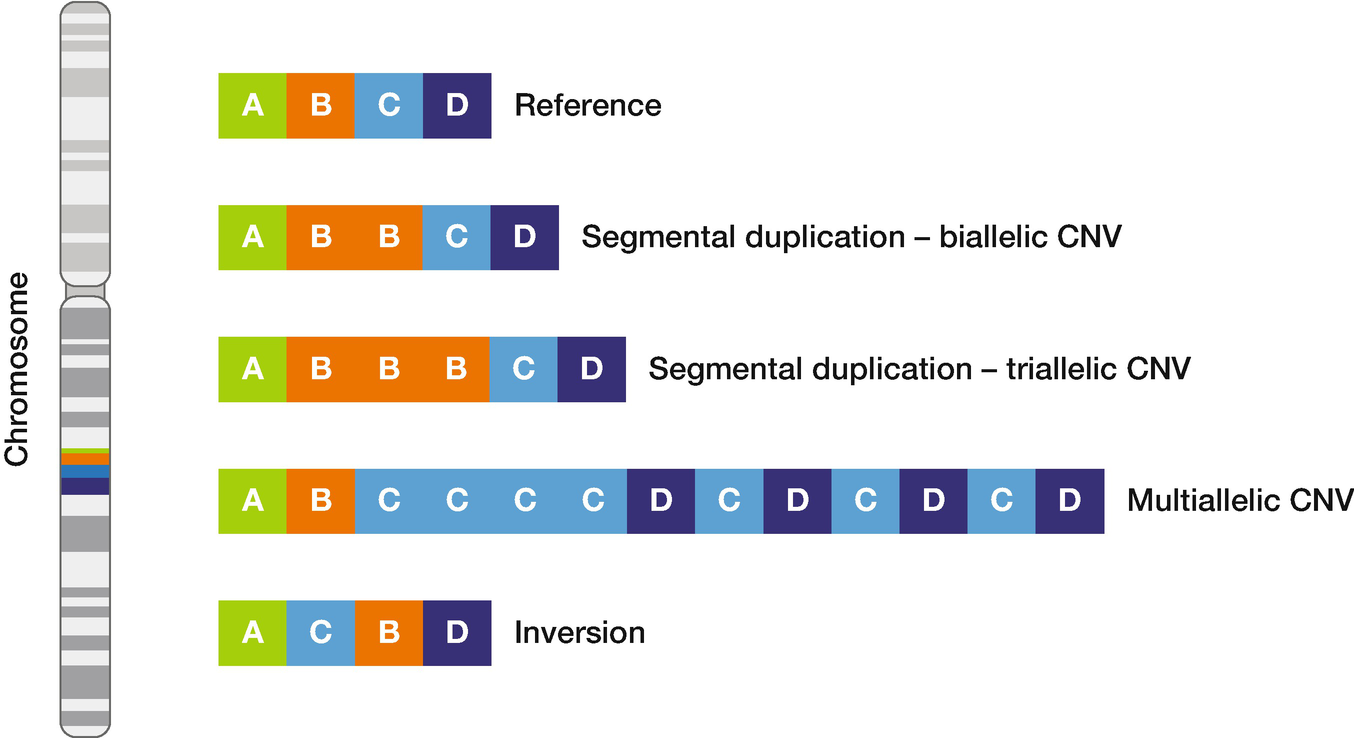
\includegraphics[keepaspectratio=true]{images/cnv.png}
		\caption{Основные типы структурных вариаций}
	\end{figure}
	Разновидности структурных вариантов на этом не исчерпываются, но в контексте данной работы наибольший интерес представляет число копий крупных фрагментов генома. Такого рода структурные вариации характерны для опухолевых клеток.
\end{definition}

\begin{definition}[\textit{Медуллобластома}]
	Самый распространённый тип педиатрической опухоли мозга. Поражает мозжечок.
	\begin{figure}[H]
		\centering
		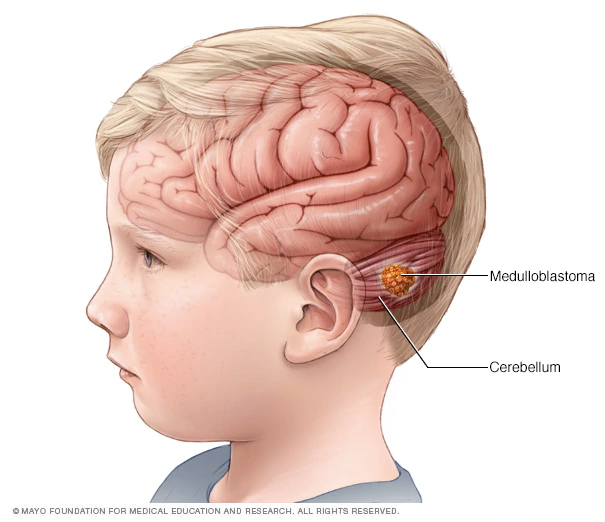
\includegraphics[keepaspectratio=true, scale=0.4]{images/medulloblastoma.png}
	\end{figure}
\end{definition}

\begin{definition}[\textit{Хромотрипсис}]
	Мутационный процесс, в ходе которого тысячи локальных структурных вариаций случаются в небольших фрагментах генома, локализованных в одной или нескольких хромосомах. Играет важную роль в онкогенезе в отдельных типах рака и в появлении некоторых врождённых заболеваний.
	\begin{figure}[H]
		\centering
		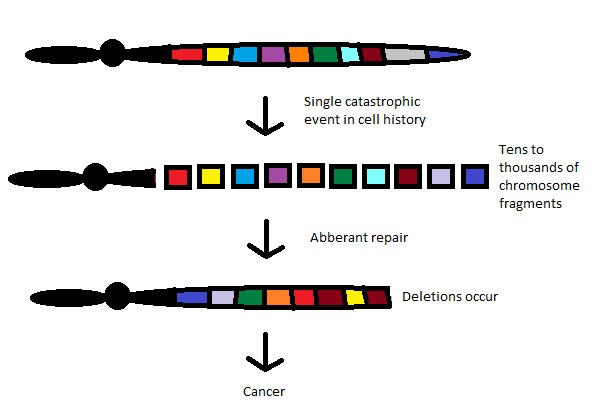
\includegraphics[keepaspectratio=true, scale=0.7]{images/chromothripsis.png}
		\caption{Хромотрипсис}
	\end{figure}
\end{definition}

\begin{definition}[\textit{Клональная линия}]
	Класс эквивалентности клеток по отношению схожести генного материала в них. Конкретное определение этой "схожести" зависит от контекста. Для того, чтобы определить понятие клональной линии в онкологии, вначале нужно дать определение \textbf{клонального события} — масштабной наследуемой мутации. К клональным событиям относят, к примеру, крупные структурные вариации, хромотрипсис, дупликацию генома, а также короткие нуклеотидные замены, которые качественно меняют фенотип клетки. 
	\begin{figure}[H]
		\centering
		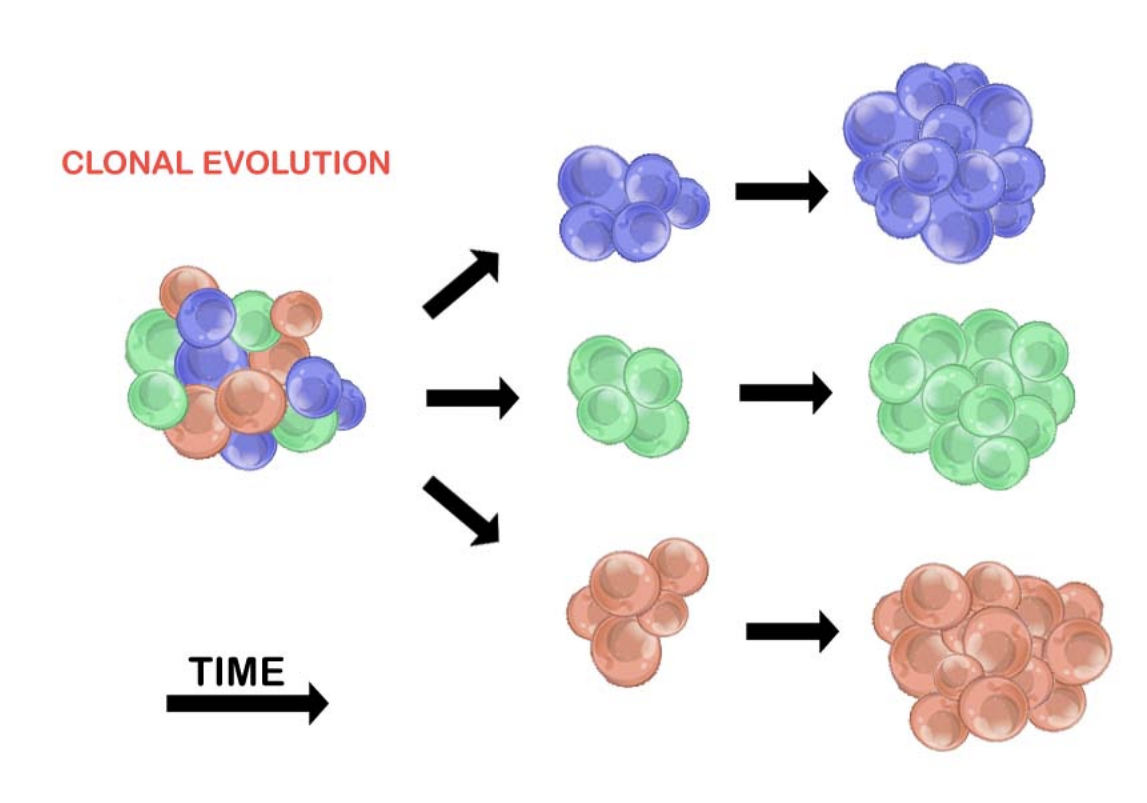
\includegraphics[keepaspectratio=true, scale=0.3]{images/tumour_clonal_structure.png}
		\caption{Клональная эволюция опухоли: клетки первичной опухоли порождают т.н клональные линии. Клетки в пределах линии генетически однородны, но клетки двух любых различных линий существенно различны.}
	\end{figure}
	Клональные события позволяют задать псевдовремя на стадиях онкогенеза. Именно \textbf{псевдо}время, т.к. клональное событие может произойти только в одной из двух произвольно выбранных генетически идентичных клеток, в связи с чем их потомки будут качественно отличаться друг от друга. Эту концепцию можно визуализировать посредством \textbf{дерева онкогенеза}, в корне которого находятся здоровые клетки, а каждое ветвление соответствует клональному событию. Тогда клональные линии можно определить как классы эквивалентности клеток, которые возникнут естественным образом, если геному каждой из них сопоставить вершину дерева онкогенеза.
\end{definition}

\begin{definition}[\textit{BAF}]
	BAF — B-Allele Frequency — нормализованная мера дисбаланса аллелей числа ридов, выравнивающихся на гетерозиготные аллели А и B. BAF, равный 0 или 1, означает полное отсутствие одного из двух аллелей, т.е. фенотип АА или BB, а BAF означает сбалансированное присутствие обоих аллелей, т.е. фенотип AB или BA.
\end{definition}

\begin{definition}[\textit{RDR}]
	Отношение числа ридов, однозначно выравнивающихся на конкретный участок генома, к ожидаемой глубине покрытия этого участка. Используется для определения числа loss и gain events в заданных сегментах генома.
\end{definition}